\chapter{Label Inference}\label{\positionnumber}
\section{Problem Statement}\label{\positionnumber}
When focusing on data objects or nodes in terms of the property graph model there is often an implicit hierarchy or taxonomy of types. Such an implicit type taxonomy may provide further insights about data as it may e.g. help in estimating cardinalities during query optimization, when keeping further statistics about the latent class distribution and may also reveal additional information about the type of instances, like how to categorize an instance, is it rare or special from a certain point view, is it an outlier, $\ldots$ In practice the categories are just informal strings, there is no notion of this structure in the current representation of the property graph model. In order to leverage this implicit taxonomy it needs to be made explicit. \\

\noindent For example businesses may be further categorized in e.g. restaurants, spas, shopping malls, etc. One may further subdivide the restaurants by additional properties and features like cooking style (Italian, Asian, burgers, $\ldots$) or by location (Italian restaurants in New York, Asian restaurants in Manhattan).
An example tag distribution is depicted in \fullref{tab:running_ex}: \\
\begin{table}[htp]
     \centering
     \begin{tabular}{c c} \toprule
            Node.name & Node.tags \\ \midrule
            Fernando's & restaurant, Italian \\ 
            Arche & restaurant, Vietnamese \\ 
            Zum Elefanten & restaurant, Thai \\ 
            Campus Cafe & cafe, WiFi \\ 
            Endlicht & cafe, late-night \\ 
            Pano & cafe, breakfast \\
            Lago & shopping, mall \\ 
            Seerhein Center & shopping, cheap \\ 
            Seepark & Shopping, expensive \\ \bottomrule
        \end{tabular}
    \caption{A fictive example of business and user-defined associated tags.}
    \label{tab:running_ex}
\end{table}{}

\noindent Which may be visualized as taxonomy like in \fullref{fig:ex_hier}. \\
\fig{img/ex_hierarchy}{ex_hier}{The taxonomy that is implicit in the tags of the example in \fullref{tab:running_ex}}{1} \\
 
\noindent \textbf{Problem:} Given a Property Graph  $G = (V, E, \lambda, P, T, L, f_P, f_T, f_L)$, we aim at extracting a taxonomy inducing a set of meaningful labels with the following extracted information:
\begin{itemize}
    \item the user-defined labels of the nodes $V, L, f_l$ and types of the relationships $E, T, f_T$,
    \item the properties of the nodes and relationship $V, E, P, f_P$,
    \item per node structural features of the underlying graph that is the node degree, the average neighbour degree, the number of nodes incoming to the ego net and the number of nodes outgoing from the ego net and
    \item the characteristic set of a node, that is the set of all relation types associated with this node.
\end{itemize}

\section{Proposed Solution}
Finding classes or in other terms subsets of the input is what is addressed by clustering methods. Extracting a hierarchy of classes is what hierarchical clustering copes with (see \fullref{3.1}). \\

\fig{img/pipeline.png}{pipeline}{The pipeline that is used to generate the taxonomy.}{1}


\subsection{Pre-Processing}\label{\positionnumber}
\subsubsection{Encoding Sets of Tags as Vectors}
\begin{algorithm}[htp]
    \KwIn{Set of Objects $O$, set of sets of Attributes $A = \{A_{o_0}, A_{o_1}, \dots \}$}
    \Parameters{No Parameters}
    \KwOut{A matrix $M$ of shape $|O| \times |A|$ with $m_{o,a} \in \{0, 1\}$} 
    \Begin{
        $M \rightarrow zeros(|O|, |A|)$\;
        \For{Object o in O} {
            \For{Attribute a in A}{
                \If{$a \in A_o$}{
                    $M[o,a] = 1$\;
                }
            }
        }
    }
\caption{Vectorize tags}\label{vect}
\end{algorithm} 
\noindent After loading the data it needs to be converted into a representation that the clustering algorithms work on. Most clustering algorithms take a feature vector as input, that is a matrix of real numbers on some metric space. The only exception to this is conceptual clustering \fullref{3.4}. Character strings need to be transformed to comply with this requirement. Text Vectorization, also referred to as One-Hot encoding builds a matrix representation, given a set of string attributes per object.

\noindent Consider the example given in \fullref{tab:running_ex}. The vectorized representation of the example in table \fullref{tab:running_ex} is given in \fullref{tab:vect_running_ex}
\begin{table}[htp]
     \centering
     \begin{tabular}{|c|c|c|c|c|c|c|c|c|c|c|c|c|} \hline
            Node.name & rest & ital & viet & thai & cafe & wifi & late & brea & shop & mall & chea & expe \\ \hline \hline
            Fernando's      & 1 & 1 & 0 & 0 & 0 & 0 & 0 & 0 & 0 & 0 & 0 & 0  \\  \hline
            Arche           & 1 & 0 & 1 & 0 & 0 & 0 & 0 & 0 & 0 & 0 & 0 & 0  \\  \hline
            ZumElefanten    & 1 & 0 & 0 & 1 & 0 & 0 & 0 & 0 & 0 & 0 & 0 & 0  \\ \hline
            CampusCafe      & 0 & 0 & 0 & 0 & 1 & 1 & 0 & 0 & 0 & 0 & 0 & 0 \\ \hline
            Endlicht        & 0 & 0 & 0 & 0 & 1 & 0 & 1 & 0 & 0 & 0 & 0 & 0 \\ \hline
            Pano            & 0 & 0 & 0 & 0 & 1 & 0 & 0 & 1 & 0 & 0 & 0 & 0 \\ \hline
            Lago            & 0 & 0 & 0 & 0 & 0 & 0 & 0 & 0 & 1 & 1 & 0 & 0 \\ \hline
            Seerhein Center & 0 & 0 & 0 & 0 & 0 & 0 & 0 & 0 & 1 & 0 & 1 & 0 \\ \hline
            Seepark         & 0 & 0 & 0 & 0 & 0 & 0 & 0 & 0 & 1 & 0 & 0 & 1\\ \hline
        \end{tabular}
    \caption{A vector representation of the example from \fullref{tab:running_ex} corresponding to $I$}
    \label{tab:vect_running_ex}
\end{table}{} \\

\subsubsection{Feature Vector Extension}
Here we take the full complexity of available information into account: Categorical values as before, numerical values, graph structure and a few label-based semantic features using a graph database (Neo4j) employing the property graph model.
As we focus on a label hierarchy we want to extract structural features from the nodes (compare with \fullref{2.1}: Nodes have labels, relationships have a type).
When no properties are present at all then structural features are the information that can be extracted. Following the approach of Henderson et al. and Neumann et al. described in \fullref{3.5} the features that are extracted are
\begin{itemize}
    \item the degree of the node,
    \item the average neighbour degree,
    \item the amount of relationships that are outgoing from the ego net,
    \item the amount of relationships that are incoming to the ego net and
    \item the characteristic set.
\end{itemize}
As the proposed method shall be a proof of concepts, the extracted features are neither complete nor exhaustive. Additionally weighted, directed and recursively aggregated versions of the above should also be considered.
Note that more semantic or concept-based features can be extracted, like aggregated neighbour property concepts or regarding relationships what node property types are connected by a certain edge concept. Also less features overall may provide better results as the priority of the more important features is reduced by adding more features in an unweighted feature vector. \\


\subsection{Clustering}\label{\positionnumber}
The methods described in \fullref{3.1.1}, \fullref{3.1.2}, \fullref{3.3.3} and \fullref{3.4.1} already produce hierarchies as outputs, so those methods may be applied to the pre-processed data without further clustering steps. All other approaches produce only ``flat`` clusters. Similarly to HDBSCAN, one can apply hierarchical clustering to overcome weaknesses of both approaches: The resource requirements of hierarchical clustering algorithms are less when it is applied to the input, that was clustered before with a more efficient clustering method. In order to do this, we first apply a non-hierarchical algorithm to the input data set. Then for each cluster take the intersection of the set of tags of all objects in the cluster in order to obtain a class description for all clusters. On those newly formed objects perform hierarchical clustering to generate a hierarchy. This comes with the obvious cost of loss of information, and is especially difficult when data is noisy. Problems and ways to overcome those are discussed in \fullref{5}. \\
Further many clustering algorithms have parameters that need to be optimized for the data set, e.g. for k-Means the number of clusters needs to be known in advance. \\

\noindent Applying the proposed algorithms to the extended feature vector yields something similar to Henderson's role extraction~\cite{henderson2012rolx}, but with additional information: Not only the role is analyzed but also the characteristics of the object itself. What is captured as concepts in the hierarchy or taxonomy constructed depends on the concrete feature vector that is chosen: The labels a node has and what labels occur together, the distribution over the properties a node has, what type the relations are (characteristic set), how it is embedded into the graph in terms of structure. \\
Returning to the road network example this would classify the crossings by the street types and their properties, meaning that a motor way junction (a few wide long streets crossing) should end up in a different concept than a country road crossing (a few long but not too wide streets crossing). \\
From a theoretical point of view the proposed method is able to deal with object-oriented data, triplets like in RDF and a mixture of both models, that is the property graph model. It is able to summarize information and extract probabilistic concepts from relations, components and thereof constructed objects and graphs in a parameter-free and unsupervised manner. 


\subsection{Post-Processing: Taxonomy Extraction}\label{\positionnumber}
Applying hierarchical agglomerative clustering on the results of the previously applied algorithm yields a hierarchically ordered set of subsets of $O$ but with only one merge per tree depth level: This is a characteristic trait of a dendrogram and the most significant difference to other trees and tree-like structures. Instead of consisting of only $\log_k n$ levels it consists of $n$ levels. Thus the dendrogram can be flattened to get the corresponding ``well-formed`` tree of clusters - a taxonomy. \\
The output of agglomerative clustering is a linkage matrix, a matrix of shape $3 \times |merges|$, where column 0 contains the first merged cluster, column 1 the second merged cluster and column 2 the distance of the merged clusters, representing the hierarchically ordered set of subsets.
What the flattening intuitively does is aggregating merges where clusters have been merged consecutively and with the same distance. \\
An example input and output pair is shown in \fullref{fig:my_label}.
\begin{algorithm}[htp]
    \KwIn{linkage matrix $lM$}
    \Parameters{None}
    \KwOut{A taxonomy of $O$} 
    \Begin{
        previousRow $\leftarrow [-1, -1, -1]$\;
        taxonomy $\leftarrow$ new Map\;
        cluster $\leftarrow$ new Set\;
        distance $\leftarrow$ -1\;
        consecutive = False\;
        \For{row in $lM$}{
            \If{(row[0] == previousRow[0] or row[1] == previousRow[1])  and row[2] == previousRow[2]}{
                \If{taxonomy is not empty and not consecutive}{
                    taxonomy.removeLast()\;
                    cluster.add(previousRow[0], previousRow[1])\;
                }
                 distance $\leftarrow$ row[2]\;
                 cluster.add(row[0], row[1])\;
                 consecutive $\leftarrow$ True\;
            }{
                \If{consecutive}{
                    taxonomy.add(clusters, distance)\;
                    cluster.clear()\;
                    distance = -1\;
                }
                consecutive = False\;
                taxonomy.add(\{row[0], row[1]\}, row[2])
            }
        }
        return cluster
    }
\caption{Taxonomy Extraction from a Dendrogram}\label{taxo}
\end{algorithm}

\begin{figure}[htp]
    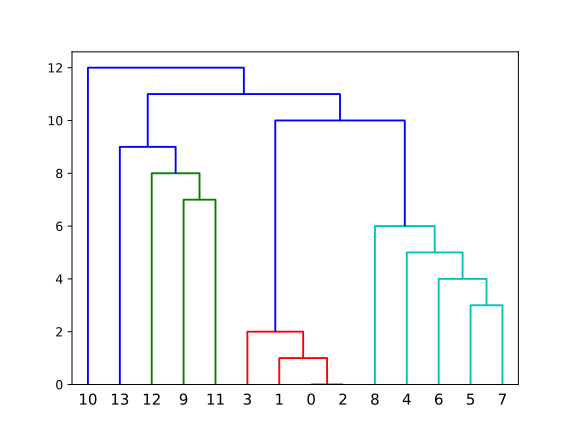
\includegraphics[width=0.49\textwidth]{img/extract_ex_dendro.png}
    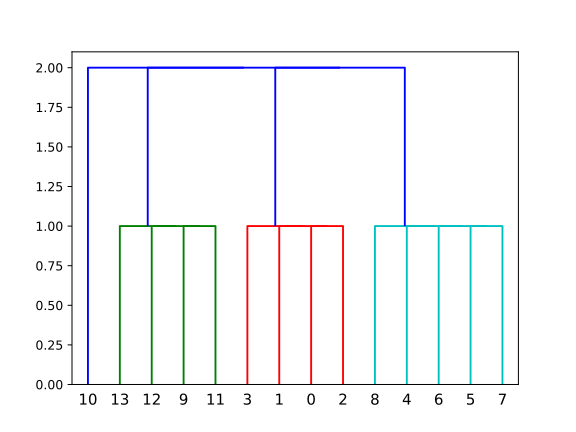
\includegraphics[width=0.49\textwidth]{img/extract_ex_taxo.png}
    \caption{The Input and output of the taxonomy extraction heuristic}
    \label{fig:my_label}
\end{figure} 
